\section{问题一：能源现状与协同潜力}
\subsection{历史总量、结构与电源演化}
历史窗口为2010—2024年，能源生产与消费采用《中国统计年鉴2025》同版次资料\cite{nbs_yearbook_2025_9_2,nbs_yearbook_2025_9_1}；电源装机和分技术发电分别使用国家统计局连续序列与Ember历史面板\cite{ember_latest_2026_10_16}，各自在原统计口径内分析。GDP为世界银行2015年不变美元序列\cite{worldbank_NY.GDP.MKTP.KD}，燃料CO$_2$为GCB经OWID整理的煤、油、气和放空分项\cite{owid_gcb_2025}。

\begin{figure}[H]\centering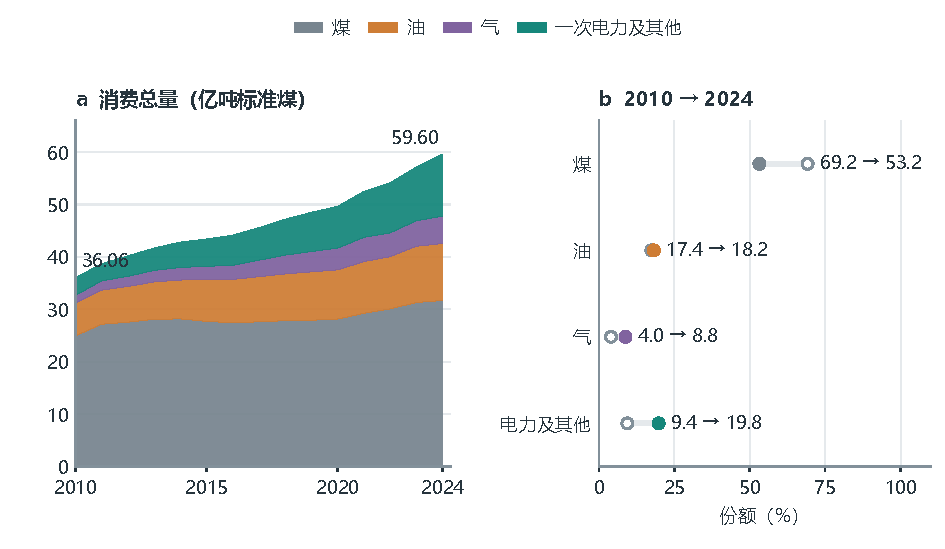
\includegraphics[width=\linewidth]{figures/fig00a_observed_consumption.pdf}\caption{同版年鉴下的一次能源消费规模与结构演变。}\label{fig:fig00a_observed_consumption}\end{figure}

\begin{figure}[H]\centering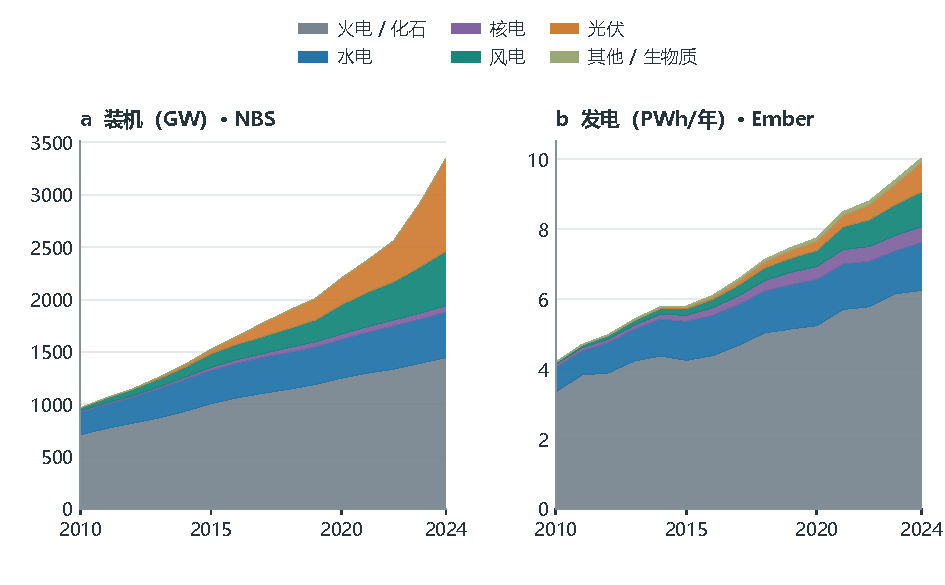
\includegraphics[width=\linewidth]{figures/fig00b_observed_power.pdf}\caption{电源装机与发电结构在各自连续统计口径内的演变。}\label{fig:fig00b_observed_power}\end{figure}

2024年一次能源消费为 5,960 Mtce，煤、油、气及“一次电力及其他能源”份额分别为53.2\%、18.2\%、8.8\%与19.8\%。历史图保留这一原始分类。Ember口径电力总需求为10069.88 TWh，国家能源局全社会用电量9852.1 TWh另按其消费端定义记录\cite{nea_electricity_2024}。电力作为二次能源，在总量核算中与发电燃料分别处理；宏观一次电力折标遵循能源平衡口径\cite{nbs_energy_method,nbs_energy_faq}。

2010—2024年一次能源消费增长65.3\%，同期实际GDP指数增长139.7\%。燃料相关CO$_2$由7.865升至11.485 Gt，增加46.0\%；2024年风光发电占比为18.3\%。能源规模增长与化石份额下降同时发生，说明结构改善需要与总量、效率和服务交付一起评价。
赛题附件1—4给出火电、水电、抽蓄、风电与核电五类电站名录，分别含633/193/31/16/17条非空记录\cite{official_station_lists}。名录的参考年份与抽样设计未声明，部分表存在重复记录，且只有抽蓄与风电提供经纬度。本文保留原始名录，用于核对给定场站规模与空间分布；全国年度总量、结构和模型初态采用上述连续统计序列，避免把名录容量直接替代全国装机。

\subsection{燃料供应、价格与区域分布}


\begin{figure}[H]\centering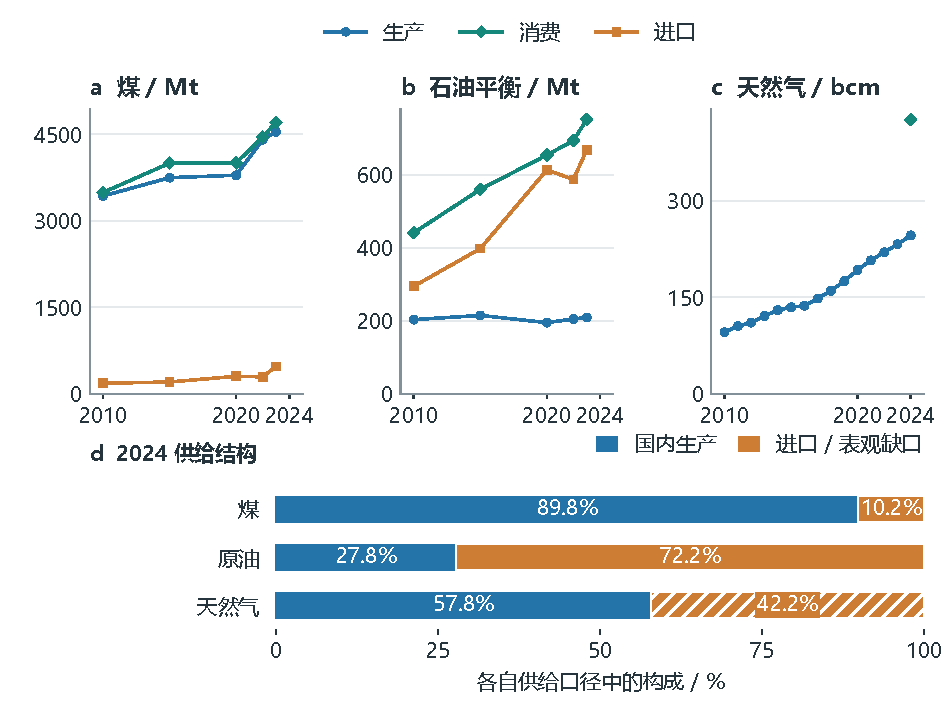
\includegraphics[width=\linewidth]{figures/fig00c_fuel_balance_exposure.pdf}\caption{三燃料历史供需与2024年供给结构。a—c保持Mt与bcm原始量纲，煤、油仅连接选定观测年，气消费仅显示2024年点。d的煤、原油比例分别以国内生产加进口为分母，气以表观消费为分母，斜纹段表示消费减生产的表观缺口。上排石油平衡含成品油贸易，下排使用原油生产与进口；气表观缺口不等同总进口。}\label{fig:fig00c_fuel_balance_exposure}\end{figure}

煤及褐煤、原油、成品油的2024年进口分别为542.70、553.42、48.23 Mt\cite{nbs_communique_2024}；天然气总进口181.7 bcm，由管道气76.0与LNG气化体积105.7 bcm构成\cite{nea_gas_development_2025}。三种燃料进口均作为独立渠道，库存、直接使用和发电领用按各自燃料守恒。

煤原料供应集中于晋陕蒙，天然气集中于西部产区，水电集中于西南。按年鉴全国总量作分母，煤前三产区约占70.30\%，天然气前三约58.37\%，水电前三约60.71\%\cite{nbs_yearbook_2025_9_19}。这种空间差异说明，能源品种的互补需要同时考虑料源、输送与灵活性。

\begin{figure}[H]\centering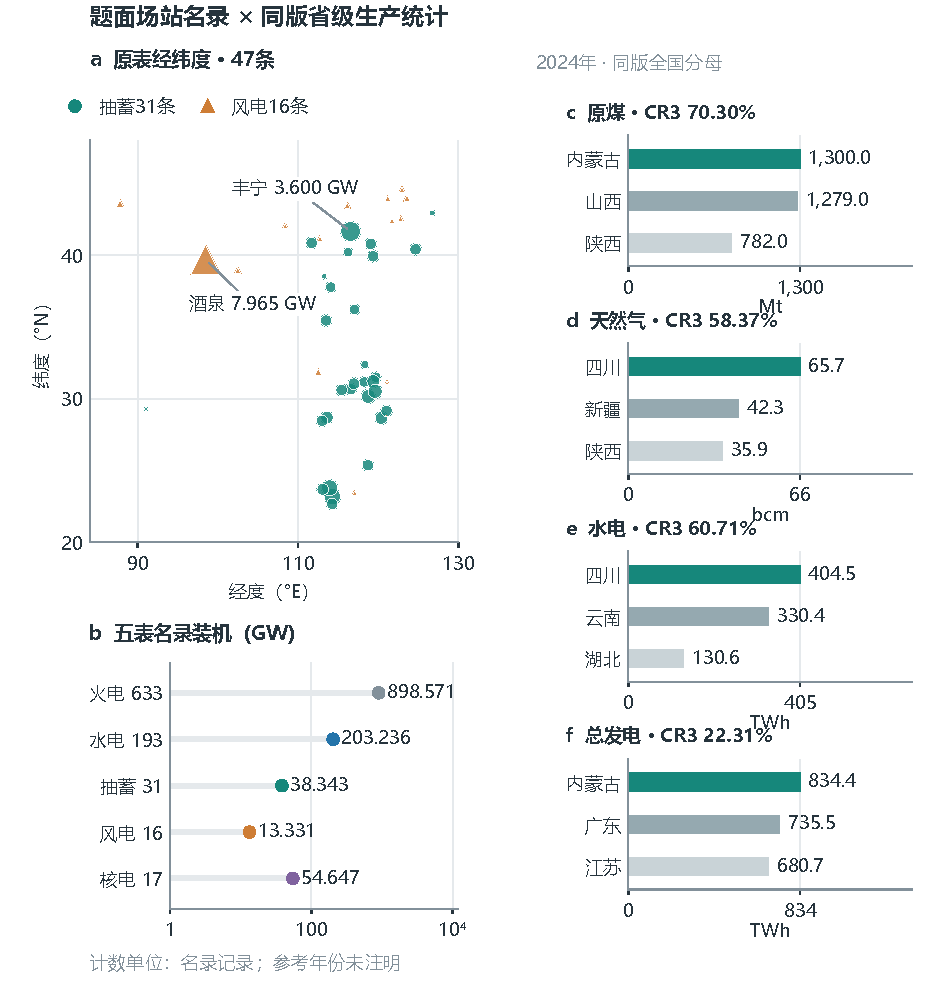
\includegraphics[width=\linewidth]{figures/fig00e_observed_regions.pdf}\caption{题面电站名录与2024年省级生产集中度。左上按附件原值绘制47条经纬度记录，点面积与装机成正比，坐标图不含行政边界；左下汇总五张表全部890条名录记录，火电、水电、核电843条未提供坐标。右侧四组沿用同版年鉴的全国分母和前三省原值。名录参考年份未注明，同名与重复记录保留，装机合计不代表2024年全国总量。}\label{fig:fig00e_observed_regions}\end{figure}

经济性以工程资本与燃料资源账分别评价。2024年12月下旬5500大卡煤767.9元/吨、LNG4413.8元/吨为流通领域价格快照\cite{nbs_prices_2024_dec_late}；长期技术资本系数采用工程参数。生物质2024年以45.99 GW和208.3 TWh成套资料建立初态\cite{nea_renewable_2024}。氢能总产量超过36.5百万吨、已建可再生电解水产能约0.125百万吨/年\cite{nea_hydrogen_2025}，纳入现状研判；本次动态模型重点评价电源、储能与三燃料交付。

现状的主要矛盾是化石燃料仍承担高比例服务、新能源发电快速增长、料源与可用出力存在空间和时间错配。协同方向对应三类资源：建设端提前形成可靠能力，运行端利用储能和服务偿还协调波动，保障端按煤油气分别维护进口渠道与库存。

\subsection{多能源发展现状的四维定量评价}
供给保障、清洁低碳、经济性与协调性分别对应不同物理量。表\ref{tab:current-four}以同口径事实识别优势与约束，再将其转为后续主体和资源规则。
\begin{table}[H]\centering\caption{2024年现状的四维定量证据与协同方向}\label{tab:current-four}
\begin{tabularx}{\linewidth}{p{.14\linewidth}p{.42\linewidth}X}\toprule
评价维度 & 定量证据 & 优势、约束与协同方向\\\midrule
供给保障 & 煤、原油进口占生产加进口分别10.2\%、72.2\%；气表观供给缺口占42.2\% & 煤具有国内供应基础，油气渠道暴露较高；按品种配置国内能力、进口与库存\\
清洁低碳 & 煤消费份额由2010年69.2\%降至53.2\%；风光发电占18.3\% & 结构改善与总量增长并存，评价排放同时检查服务交付\\
经济性 & 2024年12月下旬5500大卡煤767.9元/吨、LNG4413.8元/吨 & 分别记录燃料价格快照；工程资本、运行资源费和采购现金独立核算\\
时空协调 & 煤、气、水电前三产区占全国分别70.30\%、58.37\%、60.71\% & 料源集中与电源时序差异并存；建设工期、小时出力及资源准备共同检验\\
\bottomrule\end{tabularx}\end{table}
历史“一次电力及其他能源”19.8\%沿用年鉴原分类；前瞻模型的非化石份额另按七类电源形成。燃料吨价在各自品种和统计时点内解释，不将不同热值品种的吨价直接当作供能经济性排序。

\begin{table}[H]\centering\caption{现状证据如何进入协同模型}
\begin{tabularx}{\linewidth}{p{.14\linewidth}XX}\toprule
能源环节 & 优势与主要约束 & 模型中的实际处理\\\midrule
煤炭 & 承担主要服务，燃烧排放与料源集中并存 & 国内/进口分账，直接使用与发电竞争同一库存\\
油气 & 载能用途独立，跨境供给影响资源准备 & 两类独立进口、库存与直接服务，天然气另进入发电\\
风光 & 发电占比增长，可用出力随时段变化 & 建设订单经工期形成装机，小时可用率约束交付\\
水核生物质 & 补充稳定出力，分别受工期、来水及料源制约 & 工期队列、外生水电可用率与生物质料源预算\\
储能与移峰 & 重分配交付时点，作用受功率、能量与偿还期限约束 & 两类SOC守恒、充放功率上限与服务债务归还\\
氢能 & 可再生电解水已形成产业起点，需配套链条资料 & 现状单列；本次运行模型覆盖电源、储能与三燃料服务\\
\bottomrule\end{tabularx}\end{table}
\FloatBarrier
